\documentclass{report}
\usepackage{graphicx} % Required for inserting images
\usepackage[italian]{babel}
\usepackage{tikz}
\usepackage{hyperref}
\usepackage{amsmath}
\usepackage{xcolor}
\usepackage{float}
\usepackage{soul}
\usepackage{listings} % Per evidenziare il codice

\definecolor{lightgray}{rgb}{0.9,0.9,0.9} % Definizione colore sfondo
\definecolor{darkgreen}{rgb}{0.0, 0.5, 0.0}

\lstset{
    backgroundcolor=\color{lightgray}, % Sfondo grigio
    basicstyle=\ttfamily, % Font monospaziato
    % frame=single, % Bordo attorno al codice
    tabsize=4, % Dimensione tabulazione
    breaklines=true, % Permette di andare a capo automaticamente
    numbers = left,
    numberstyle=\small\color{gray}
}

\title{\huge\textbf{{Refresher}}}
\date{Parte I}

\begin{document}

\maketitle
\tableofcontents
\newpage


\chapter{Basics}

\section{Introduzione al decision making}

Il \textit{decision making} è una parte integrante del ruolo di gestione; i dirigenti prendono centinaia di decisioni ogni giorno.

\noindent La \textit{decision science} è una disciplina che usa tecniche quantitative per il processo decisionale, ovvero suggerisce quale 
decisione prendere in base a tecniche quantitative; è usata da ricerca operativa, statistica, inforamtica \dots

\noindent Per poter applicare queste tecniche, spesso è richiesto una elaborazione dei dati grezzi in dati elaborati per ottenere un risultato.

\noindent Il decision making ha 3 proprietà:
\begin{itemize}
    \item \textbf{Accuratezza}
    \item \textbf{Spiegabilità:} è la capacità di spiegare un risultato 
    \item \textbf{Accettabilità:} la procedura per passare dal dato grezzo al risultato è accettata da tutte le parti coinvolte
\end{itemize}

\subsection{Data exploration}
Supponiamo di avere un dataset di dipendenti, e di voler trarre una decisione sul licenziare o meno un dipendente in base all'assenteismo; vogliamo 
trarre delle informazioni dai dati usando delle semplici \textit{statistiche descrittive}. 

\noindent Nel nostro dataset troveremo sia dati \textbf{categorici} (etichette) che \textbf{numerici}.

\subsubsection{Bucketizzazione}

È un'operazione che permette di trasformare un dato numerico in uno categorico: l'insieme dei valori viene suddiviso in intervalli disgiunti; 
successivamente, ciascun valore viene sostituito con l'etichetta del suo intervallo.

\subsubsection{Istrogammi e distribuzione}
Una volta fatta la bucketizzazione, è più facile la visualizzazione grafica della distribuzione dei dati tramite istogrammi.

\begin{figure}[H]
    \centering
    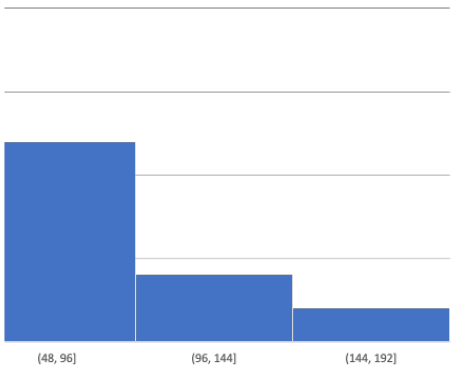
\includegraphics[width=0.5\linewidth]{images/isto.png}
\end{figure}

\subsubsection{Deviazione standard campionaria}
La deviazione standard misura quanto i valori numerici di una caratteristica sono dispersi rispetto alla media.

\noindent Se il grafico ha una forma a campana simmetrica:
\begin{itemize}
    \item $\sigma$ piccola indica valori vicini alla media 
    \item $\sigma$ grande indica valori lontani dalla media, valori dispersi 
\end{itemize}

\begin{figure}[H]
    \centering
    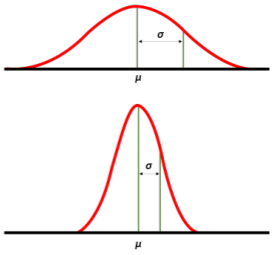
\includegraphics[width=0.5\linewidth]{images/deviazione-standard.png}
\end{figure}

\noindent La formula prevede di calcolare la varianza di ciascun valore (distanza dalla media al quadrato) divisa per il numero di valori, il tutto 
sotto radice.

\subsubsection{Mediana}

La mediana è quel valore che divide l'insieme a metà; è quel valore per cui il 50\% dei valori è più piccolo e l'altro 50\% è più grande.

\subsubsection{Quartili}
\begin{itemize}
    \item \textbf{Primo quartile:} valore $x$ tale che 25\% dei valori è minore di $x$
    \item \textbf{Secondo quartile:} valore $x$ tale che 50\% dei valori è minore di $x$
    \item \textbf{Terzo quartile:} valore $x$ tale che 75\% dei valori è minore di $x$
\end{itemize}

$\Rightarrow$ il secondo quartile coincide con la mediana 

\noindent La \textbf{differenza interquartile} (differenza tra terzo e primo quartile) è utile per fare analisi su dati la cui distribuzione non è 
a campana simmetrica, dato che la deviazione standard ha senso di essere usata solo su dati che seguono quella distribuzione (altrimeniti la 
media non sarebbe un valore tipico, non avrebbe senso misurare la distanza da essa).

\subsection{Relazione tra due feature}

Ci si può chiedere se due colonne di un dataset siano correlate, ovvero se sono legate a tale punto che mi basta saperne una per conoscere anche l'altra.

\noindent Si possono mettere le due caratteristiche su un piano e rappresentarle graficamente per vedere se esiste una correlazione:

\begin{figure}[H]
    \centering
    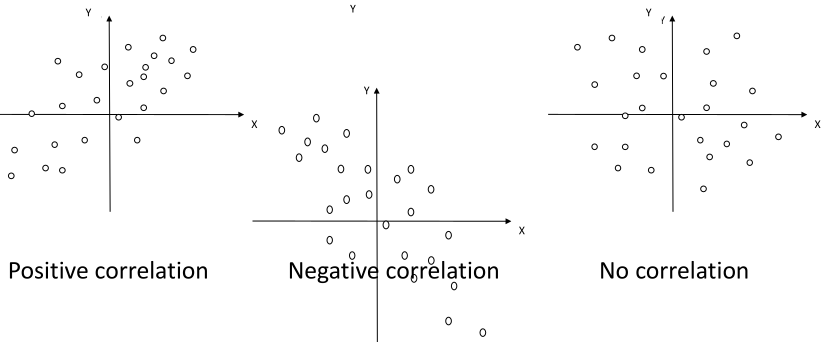
\includegraphics[width=1\linewidth]{images/correlazione.png}
\end{figure}

\noindent È possibile usare due metriche:
\begin{itemize}
    \item \textbf{Varianza:} dà informazioni sulla variabilità interna di una variabile 
    \item \textbf{Covarianza:} dà informazioni su come due variabili variano insieme; mi dice quanto il variare di una 
    influenzi il variare dell'altra
    \begin{itemize}
        \item \textit{Positiva:} le variabile variano nella stessa direzione 
        \item \textit{Negativa:} le varaibili variano nella direzione opposta
        \item \textit{Zero:} nessuna correlazione
    \end{itemize}
\end{itemize}

\noindent La covarianza viene usata per ottenere un numero tra -1 e 1 (tramite il \textit{coefficiente di correlazione di Pearson}) che mi dice quanto due variabili sono correlate tra loro.

\begin{itemize}
    \item due variabili si dicono indipendenti se non condividono informazioni 
    \item se sono dipendenti, la \textit{quantità di informazione} condivisa si stima con la correlazione
\end{itemize}

\noindent Bisogna fare attenzione a fare una distinzione tra correlazione e causa. Potrebbe sembrare che due correlazioni siano 
correlate solo perchè sono correlate ad una terza grandezza; è il caso ad esempio di suicidi e mangiare aringhe.

\subsubsection{Distribuzioni asimmetriche}
Quando un istogramma è costruito su valori che seguono una \textit{distribuzione normale}, allora la forma delle colonne sarà \textit{a campana}; 
tuttavia, in casi reali gli istogrammi sono spesso asimmetrici.

\subsection{Decision Making via algorithms}
\textit{Per quale motivo si cerca di rispondere ad un problema tramite un modello supervisionato? 
Non basterebbe avere un algoritmo?}

\noindent Gli algoritmi applicano una \textbf{teoria} alle grandezze (ad esempio la deteriorità di un motore elettrico dovuta alla temperatura); se ho una 
teoria, la posso \textbf{esplicitare con un algoritmo:} ho una funzione che lega input e output; non ho più bisogno di avere esempi, ma ho la teoria 
che mi dice che la deteriorità del motore è dovuta al numero di ore, ad una determinata temperatura\dots

\noindent Molti problemi non possono essere risolti in questo modo, dato che non c'è un'equazione esplicita; la devo \textit{tirare fuori} dall'addestramento 
del modello.


\subsection{Decision Making via Supervised Machine Learning}
Non viene usata una formula e algoritmo che descrive in modo esplicito un fenomeno per derivare l'informazione per prendere una decisione. Viene 
usata una \textbf{formula generica con dei parametri, che vengono regolati per minimizzare l'errore}. Si tratta dunque di trovare i valori 
giusti dei parametri, viene fatto nella fase di addestramento.

\noindent Viene associato a ciascun valore un peso; alla somma pesata viene poi aggiunta una costante a cui \textit{viene applicato un 
sogliatore}; in questo modo l'output è una funzione non lineare, invece che una semplice somma pesata.

\noindent La procedura di addestramento consiste nel \textbf{considerare l'errore come funzione dei pesi}, andando poi a modificarli per 
minimizzarli.

\noindent Un singolo neurone può approssimare solo una funzione lineare:

\begin{figure}[H]
    \centering
    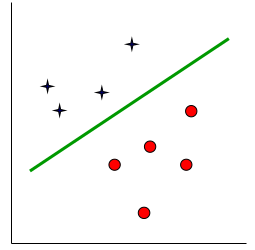
\includegraphics[width=0.4\linewidth]{images/linear.png}
\end{figure}

\noindent Una \textit{rete neurale multi-livello} può teoricamente approssimare qualsiasi funzione dopo 
una certa soglia (\textit{diventa Touring-complete}):

\begin{figure}[H]
    \centering
    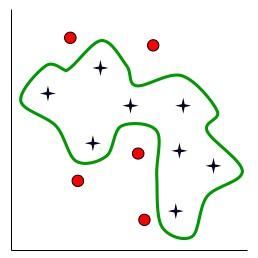
\includegraphics[width=0.4\linewidth]{images/touring-completo.png}
\end{figure}

\subsection{Ciclo di vita di un modello di ML}
L'addestramento è solo una delle parti di vita di un modello di machine learning:
\begin{itemize}
    \item \textbf{Data Management:} costruzione del dataset, controlli di vario tipo, eliminare colonne correlate tra loro \dots
    \item \textbf{Model Learning:} addestramento del modello 
    \item \textbf{Model Tuning:} fase post-addestramento in cui si danno al modello dati che non ha mai visto 
    \item \textbf{Modelo Deployment:} il modello viene messo in produzione nel caso in cui soddisfi i requisiti; altrimenti, viene 
    riportato indietro alle fasi precedenti
    \item \textbf{Model Maintenance:} si può avere un degradamento delle prestazioni perchè cambiano le distribuzioni dei dati in ingresso (è 
    preferibile che siano gaussiane e stazionarie); devo fare gli opportuni controlli 
\end{itemize} 

\noindent Ciascuna di queste fasi può subire un attacco.

\begin{figure}[H]
    \centering
    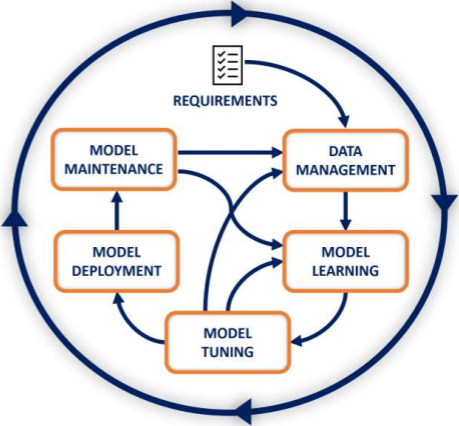
\includegraphics[width=0.6\linewidth]{images/ml-life-cycle.png}
\end{figure}


\section{Introduzione a Machine Learning}

\begin{itemize}
    \item I modelli supervisionati vanno addestrati; sono soggetti ad attacco in fase di inferenza ed in fase di training
    \item I modelli non supervisionati processano i dati sulla base delle loro proprietà, non su esempi che hanno visto; ad esempio, 
    le tecniche di clustering sono basate sulla definizione di distanze intragruppo e intergruppo. Non esiste una 
    fase di training in cui possono essere attaccati
\end{itemize}

\begin{figure}[H]
    \centering
    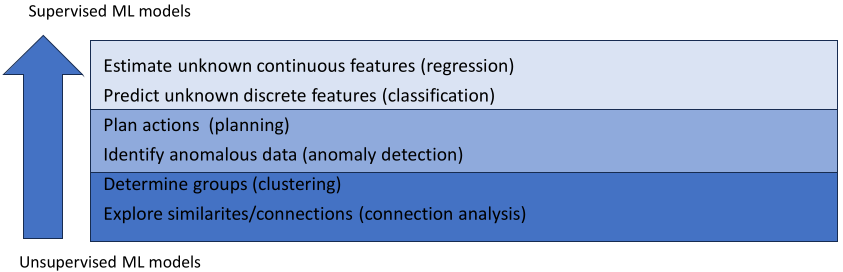
\includegraphics[width=1\linewidth]{images/intro-ml.png}
\end{figure}

\noindent Regressore e classificatore fanno parte delle task di completamento.

\subsection{Paradigma Supervised Learning}
Il problema è \textbf{imparare una relazione tra input e output a partire da degli esempi}; viene prima addestrato il modello e poi se ne ottiene uno (addestrato)
che può essere messo in produzione. In sede di addestramento il modello viene regolato per cercare di \textbf{minimizzare l'errore}.

\noindent Può essere attaccato, per cercare di violare alcune proprietà (accuratezza, ma non solo), posso cercare di fargli sbagliare un input in 
particolare, posso fare violazioni di privacy cercando se un determinato elemento appartiene al training set \dots


\noindent L'idea per creare un modello è:
\begin{itemize}
    \item viene dato un input, e il modello produrrà un output sicuramente sbagliato 
    \item si va a modificare i pesi per cercare di ridurre l'errore 
    \item si continua così fino a che ottengo dei buoni risultati che minimizzano l'errore 
    \item una volta finito questo processo, il modello non ancora pronto, perchè funziona bene sui dati che ha già visto 
    
    $\rightarrow$ devo fare una fase di testing sui dei valori che non ha mai visto (\textit{test set})
\end{itemize}

\subsubsection{\textit{Supervised ML Training in a nutshell}}
\begin{itemize}
    \item Il modello interno più semplice è una somma pesata; si ha un input multivariato, dove ogni variabile viene moltiplicata per un peso per poi
    fare la sommatoria
    \item A questa somma pesata viene poi applicata una soglia (ad esempio, se è sopra la soglia considero il risultato benigno mentre se è sotto 
    considero maligno)
    \item Quando ottengo il risultato, viene confrontato con quello reale (siamo nella fase di training), e se ho fatto un errore si va 
    a modificare i pesi cercando di diminuire l'errore
    \item Si continua tante volte in questo modo sul training set, sperando che l'errore continui a diminuire sempre di più fino a fermarmi 
    nel punto di minimo ($gradiente = 0$, ovvero la derivata delle funzioni multivariate)
\end{itemize}

\noindent All'input viene aggiunta una costante che prende il nome di \textbf{bias}, che aiuta a migliorare l'output riducendo la varianza 
e beneficiando all'accuratezza. Il training \textit{decide la quantità di bias} che massimizza l'accuratezza.

\noindent Mettendo più strati di neuroni (l'output di uno va in input ad un altro) si riesce a fare un addestramento più rapido; con 3 o più strati 
si dice che la rete è \textit{Touring completa}.

\subsubsection{Error backpropagation}
Uno dei problemi della rete neurale tradizonale è quello di non riuscire a fare una corretta \textit{error backpropagation}, ovvero non 
si riesce a distribuire l'errore anche sugli strati interni.

\noindent Per arginare questo problema si usano i primi strati per modificare la rappresentazione degli input, comprimendoli 
in una parte più piccola, mentre sono solamente gli 
ultimi quelle che vengono effettivamente addestrati.

\subsubsection{Overfitting}
Bisogna fare attenzione all'\textit{overfitting}: significa che il modello commette errore pari a 0 sui dati del training set, ma che 
su dati mai visti prima commette un grande errore; questo accade perché il modello non è in grado di generalizzare.

\noindent Per evitare che un modello vada in overfitting, generalmente un il training viene fermato prima di raggiungere un'accuratezza perfetta 
sui dati di training.


\subsection{Diversi modelli di Machine Learning}
\begin{itemize}
    \item \textbf{Classificazione:} mappa vettori di caratteristiche in \textit{categorie} o \textit{classi}
    \item \textbf{Anomaly Detection:} serve a capire se un input è anomalo rispetto a quello atteso 
    \item \textbf{Predizione:} un classificatore può anche agire da predittore, come ad esempio prevedere l'esito di un azione. Per fare il training 
    gli do sole la parte iniziale dei dati e li faccio classificare come successo/insuccesso
    \item \textbf{Planning:} sono adatti in cui non riesco a calcolare l'errore per ogni singolo input; ad esempio, se gioco a scacchi è difficile 
    classificare una singola mossa come buona o cattiva\dots

    $\rightarrow$ si usa un sistema di \textit{reward}, non calcolato sulla singola mossa ma su una sequenza di mosse
    \item \textbf{Connection Analytics:} analizza la relazione tra utenti/sistemi; fondamentale per la sicurezza (ad esempio, individuare 
    nodi centrali o vulnerabili)
\end{itemize}

\noindent $\Rightarrow$ lo stesso problema può essere risolto con modelli diversi; la scelta dipende dai dati disponibili
















\end{document}
